\documentclass{beamer}
\usepackage[spanish]{babel}
\selectlanguage{spanish}
\usepackage[utf8]{inputenc}
\usepackage{hyperref}
\usepackage{graphicx}
\usepackage{float}


\usetheme{Frankfurt}
\usecolortheme{whale}

\title{Historia de Git y sistemas de control de versión}
\author{Emmanuel Arias \href{mailto:emmanuelarias30@gmail.com}{emmanuelarias30@gmail.com}}
\begin{document}
\begin{frame}[plain]
    \maketitle
\end{frame}
\begin{frame}{Nacimiento de Git}
\begin{figure}[H]
	\centering
	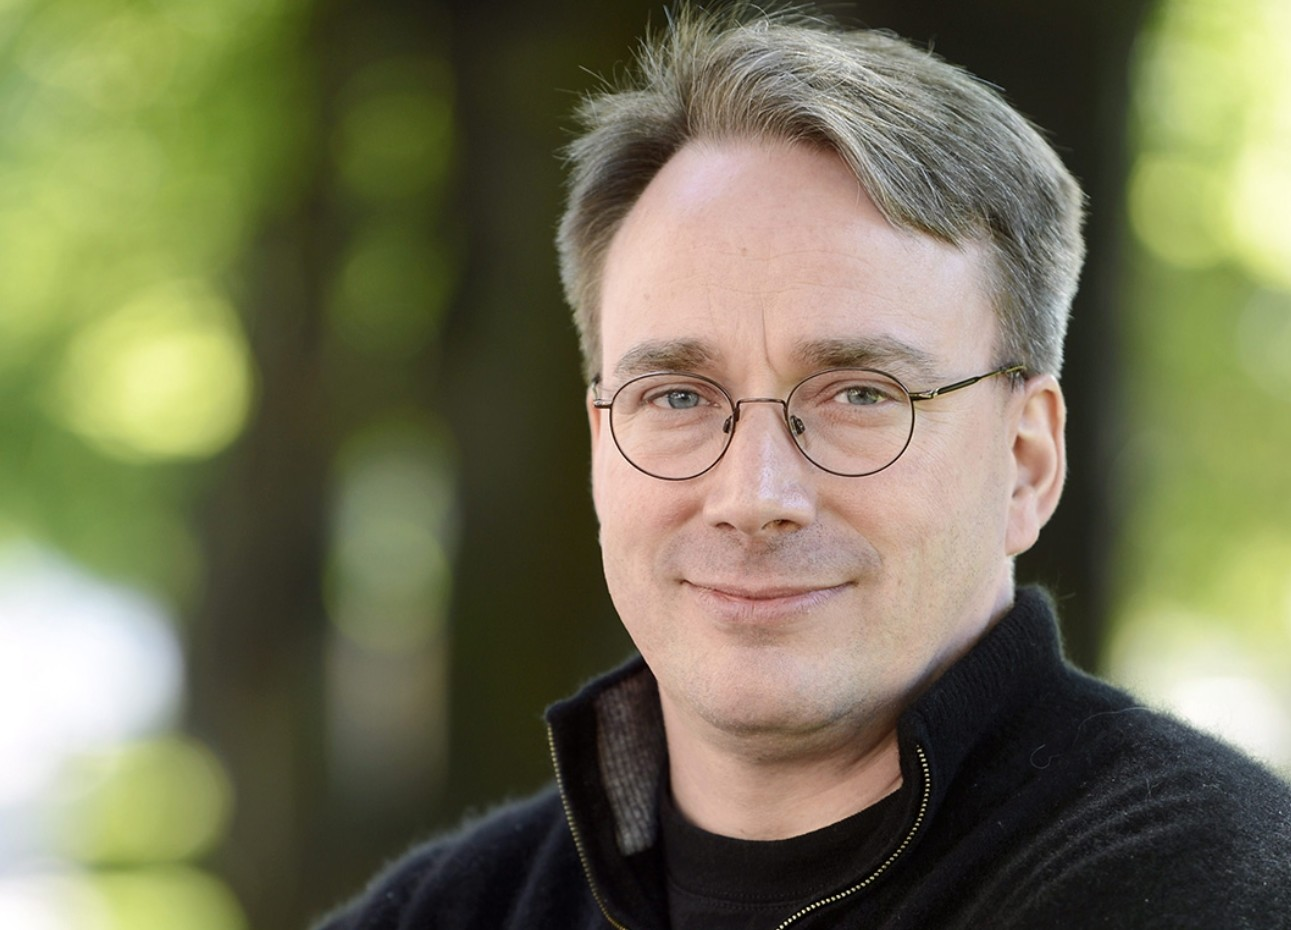
\includegraphics[width=0.7\linewidth]{img/LinusTorvalds}
	\label{fig:linustorvalds}
\end{figure}
\end{frame}
\begin{frame}{Sistemas de control de versión}
\begin{itemize}
	\item Un sistema de control de versiones es un sistema que registra todos los cambios
	que se realizan a un archivo o conjunto de ellos.
	\item Lo más importante a mencionar aquí es que estos sistemas guardan historia. Por lo que
	vamos a poder saber cómo fue evolucionando un archivo (o software) a lo largo de "la historia".
	\item Estos sistemas no son exclusivos de programadores, si no que puede ser utilizado
	por cualquiera que necesite hacer un seguimiento de los cambios realizados.
\end{itemize}	
\end{frame}

\begin{frame}
   \Huge Tipos de sistemas de control de versión
\end{frame}

\begin{frame}{Sistemas de Control de Versiones Locales}
	\begin{figure}
		\centering
		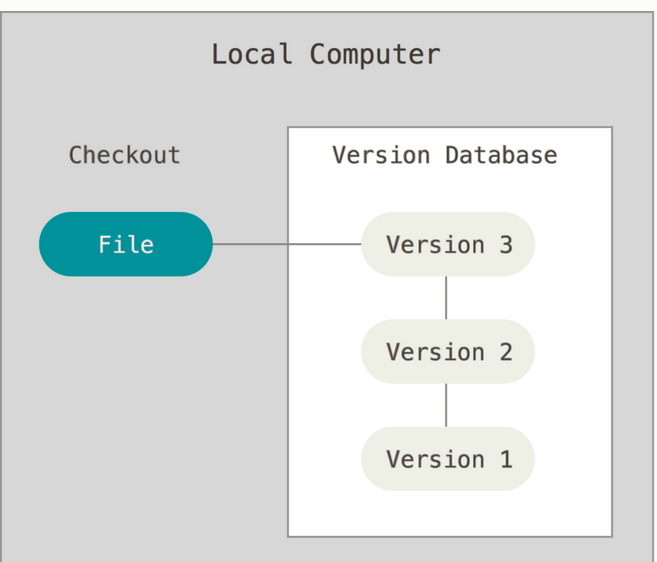
\includegraphics[width=0.7\linewidth]{img/local}
		\label{fig:local}
	\end{figure}
\end{frame}

\begin{frame}{Sistemas de Control de Versiones Centralizados}
	\begin{figure}
		\centering
		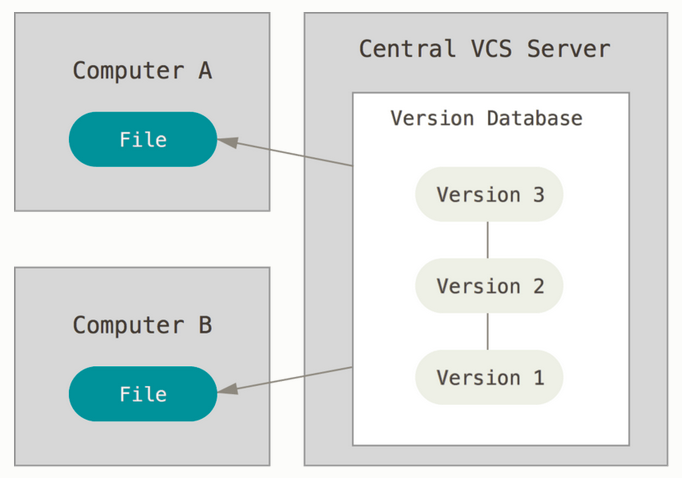
\includegraphics[width=0.7\linewidth]{img/central}
		\label{fig:central}
	\end{figure}
\end{frame}

\begin{frame}{Sistemas de Control de Versiones Distribuidos}
	\begin{figure}
		\centering
		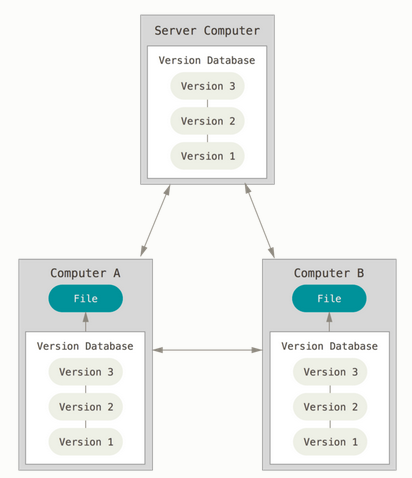
\includegraphics[width=0.7\linewidth]{img/distribuido}
		\caption{}
		\label{fig:distribuido}
	\end{figure}
\end{frame}

\begin{frame}{Git}
	\begin{itemize}
		\item Es un sistema de control de versión o sistema de gestión de código fuente. Una de las característica es que es distribuido.
		\item Es un software que permite registrar todos los cambios que se realizan en el código fuentes de cualquier proyecto.
		\item Este sistema permite comparar fácilmente diferentes versiones del proyecto, y moverse en estas.
		\item Brinda la flexibilidad de que puedan trabajar muchas personas en un mismo proyecto de eficientemente.
		\item Es un sistema distribuido por lo que no es necesario la existencia de un repositorio central (por ejemplo, svn)
		\item Permite una buena gestión de ramas y permite gestionar proyectos grandes.
		
	\end{itemize}
\end{frame}

\begin{frame}{Ventajas de Git}
	\begin{itemize}
		\item Existen múltiples repositorios redundantes y ramificaciones.
		\item Cada usuario tiene una copia completa del proyecto haciendo que el acceso a la historia sea extremadamente rápida.
		\item Puede ser utilizado con poco o sin conexión a Internet.
		\item Al ser un sistema distribuido, no hay que otorgar acceso a otras personas para que puedan utilizar las funciones de control de versiones. En vez de eso, es el dueño del repositorio el que decide a qué cambios realizar el merge y de quién.
		\item Como Git tiene el repositorio localmente no hay latencia en el trabajo, salvo cuando se requiera
		realizar push y pull.
	\end{itemize}
\end{frame}

\begin{frame}[plain]{Links interesantes}
	\begin{itemize}
		\item \href{https://www.infoworld.com/article/2670360/linus-torvalds--bitkeeper-blunder.html}{BitKeepr y Linus}
		\item \href{https://www.conasa.es/blog/git-10-anos-controlando-versiones/}{Info Git}
		\item \href{https://git-scm.com}{git scm}
		\item \href{https://www.atlassian.com/git/articles/10-years-of-git}{infografía de la historia de Git}		
	\end{itemize}
	
	
\end{frame}
\end{document}
